\documentclass{standalone}
\usepackage{tikz}
\usetikzlibrary{patterns, positioning}
\usepackage[sfdefault]{ClearSans} %% option 'sfdefault' activates Clear Sans as the default text font
\usepackage[T1]{fontenc}

\begin{document}
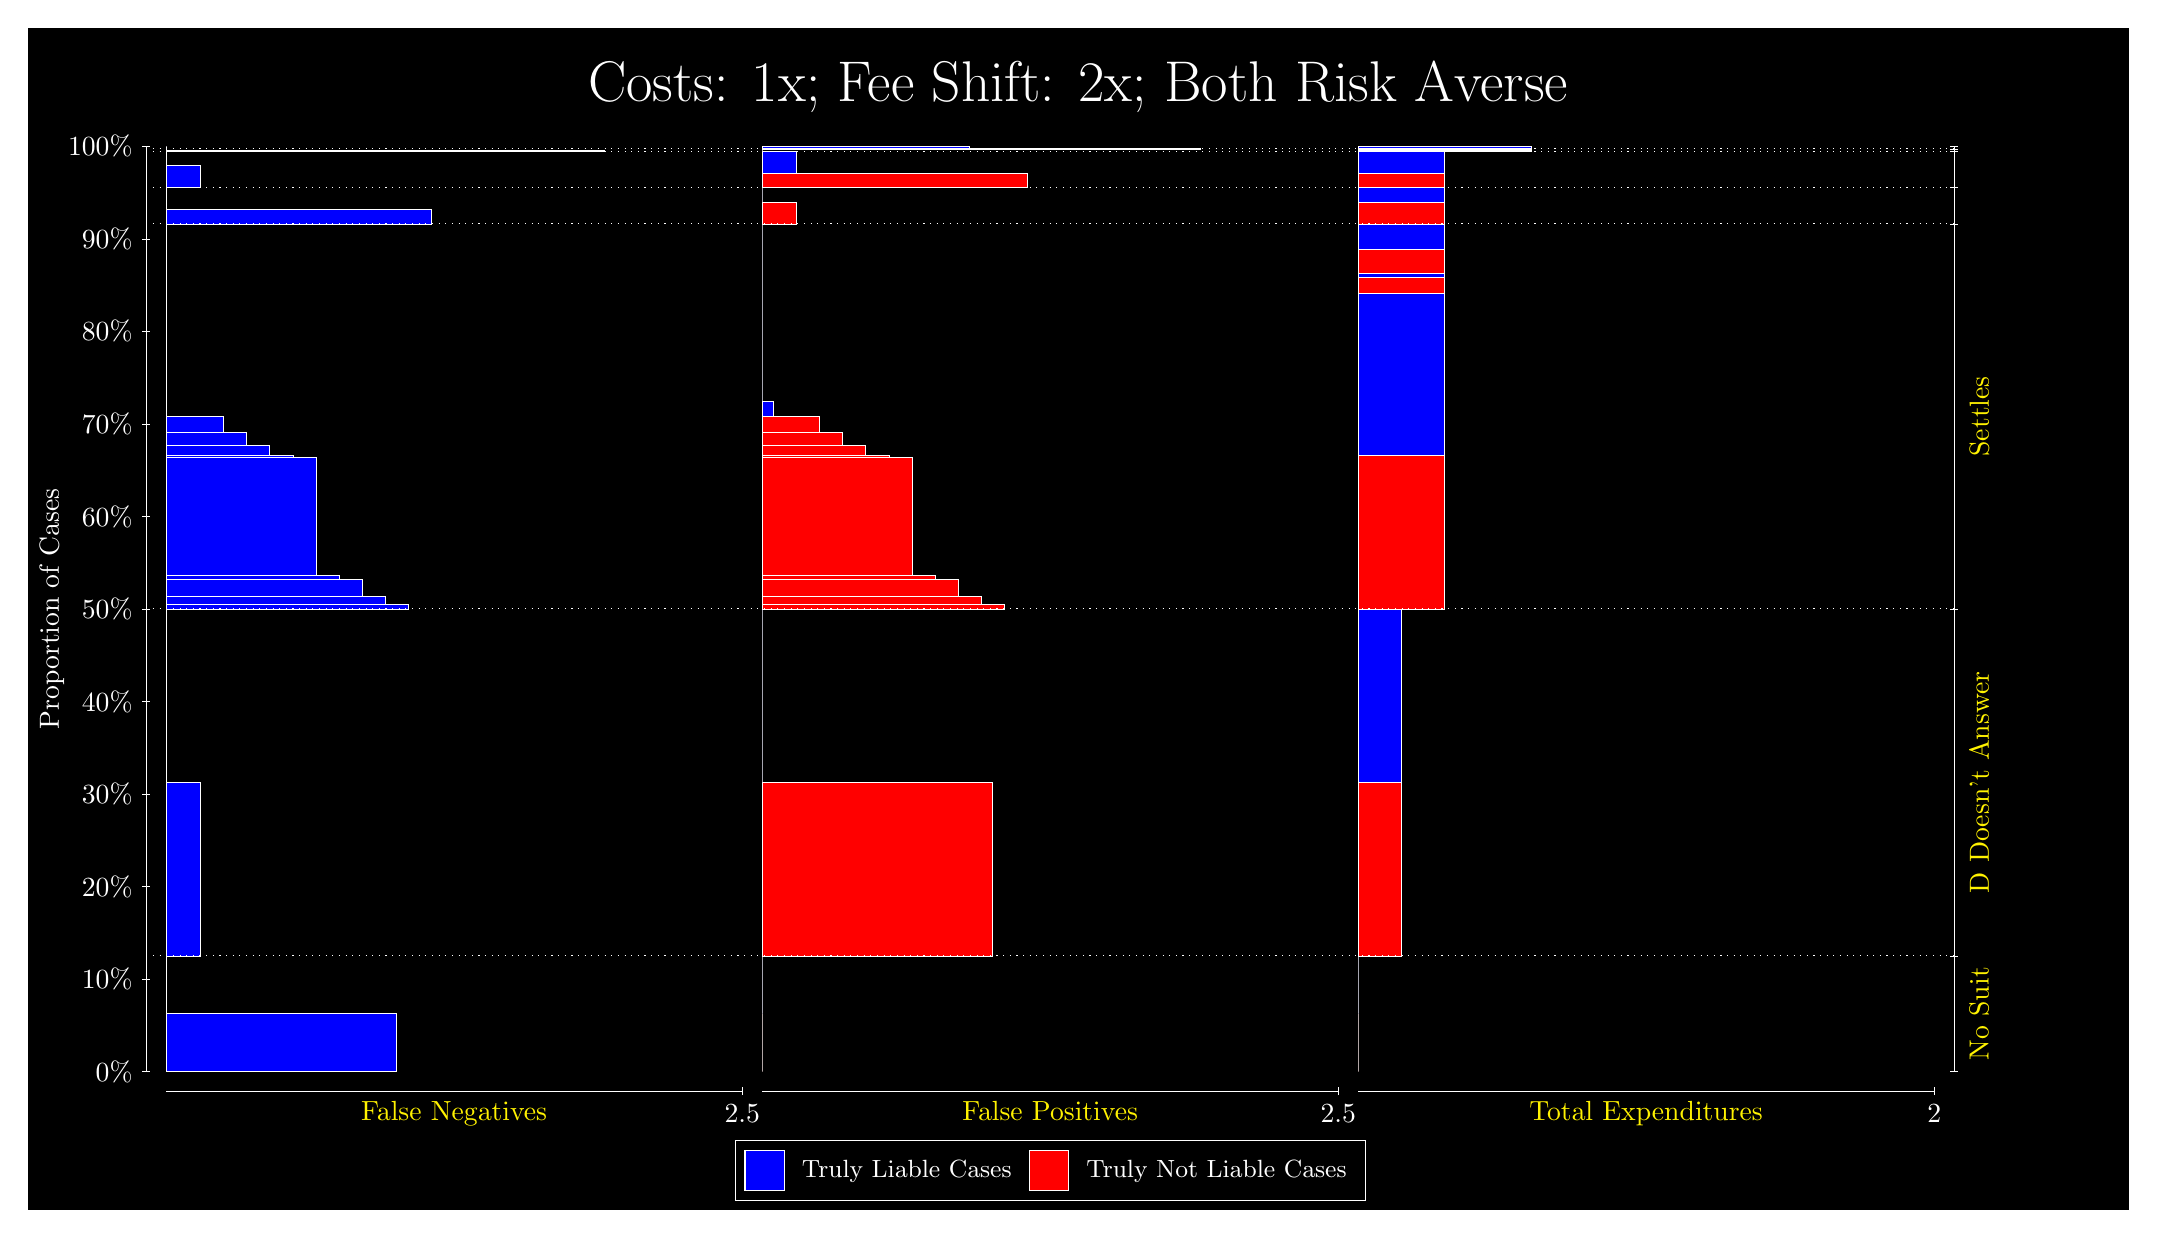
\begin{tikzpicture}
\draw[fill=black] (0,0) rectangle (26.667,15);
\draw[text=white] (0,13.5) rectangle (26.667,15) node[midway] {\huge Costs: 1x; Fee Shift: 2x; Both Risk Averse};
\draw[white, very thin] (1.5,1.75) -- (1.5,13.5);
\node[rotate=90, text=white, anchor=center] at (0.3, 7.625) {Proportion of Cases};
\draw[white, very thin] (1.45,1.75) -- (1.55,1.75);
\node[text=white, anchor=east] at (1.45, 1.75) {0\%};
\draw[white, very thin] (1.45,2.925) -- (1.55,2.925);
\node[text=white, anchor=east] at (1.45, 2.925) {10\%};
\draw[white, very thin] (1.45,4.1) -- (1.55,4.1);
\node[text=white, anchor=east] at (1.45, 4.1) {20\%};
\draw[white, very thin] (1.45,5.275) -- (1.55,5.275);
\node[text=white, anchor=east] at (1.45, 5.275) {30\%};
\draw[white, very thin] (1.45,6.45) -- (1.55,6.45);
\node[text=white, anchor=east] at (1.45, 6.45) {40\%};
\draw[white, very thin] (1.45,7.625) -- (1.55,7.625);
\node[text=white, anchor=east] at (1.45, 7.625) {50\%};
\draw[white, very thin] (1.45,8.8) -- (1.55,8.8);
\node[text=white, anchor=east] at (1.45, 8.8) {60\%};
\draw[white, very thin] (1.45,9.975) -- (1.55,9.975);
\node[text=white, anchor=east] at (1.45, 9.975) {70\%};
\draw[white, very thin] (1.45,11.15) -- (1.55,11.15);
\node[text=white, anchor=east] at (1.45, 11.15) {80\%};
\draw[white, very thin] (1.45,12.325) -- (1.55,12.325);
\node[text=white, anchor=east] at (1.45, 12.325) {90\%};
\draw[white, very thin] (1.45,13.5) -- (1.55,13.5);
\node[text=white, anchor=east] at (1.45, 13.5) {100\%};

\draw[white, very thin] (24.457,1.75) -- (24.457,13.5);
\draw[white, very thin] (24.407,1.75) -- (24.507,1.75);
\node[anchor=west] at (24.407, 1.75) {};
\draw[white, very thin] (24.407,3.2187) -- (24.507,3.2187);
\node[anchor=west] at (24.407, 3.2187) {};
\draw[white, very thin] (24.407,7.625) -- (24.507,7.625);
\node[anchor=west] at (24.407, 7.625) {};
\draw[white, very thin] (24.407,12.516) -- (24.507,12.516);
\node[anchor=west] at (24.407, 12.516) {};
\draw[white, very thin] (24.407,12.975) -- (24.507,12.975);
\node[anchor=west] at (24.407, 12.975) {};
\draw[white, very thin] (24.407,13.433) -- (24.507,13.433);
\node[anchor=west] at (24.407, 13.433) {};
\draw[white, very thin] (24.407,13.467) -- (24.507,13.467);
\node[anchor=west] at (24.407, 13.467) {};
\draw[white, very thin] (24.407,13.5) -- (24.507,13.5);
\node[anchor=west] at (24.407, 13.5) {};

\draw[white, very thin, fill=blue] (1.75,1.75) rectangle (4.6775,2.4844);
\draw[white, very thin, fill=red] (1.75,2.4844) rectangle (1.75,3.2188);
\draw[white, very thin, fill=blue] (1.75,3.2188) rectangle (2.1891,5.4219);
\draw[white, very thin, fill=red] (1.75,5.4219) rectangle (1.75,7.625);
\draw[white, very thin, fill=blue] (1.75,7.625) rectangle (4.8239,7.6789);
\draw[white, very thin, fill=blue] (1.75,7.6789) rectangle (4.5312,7.788);
\draw[white, very thin, fill=blue] (1.75,7.788) rectangle (4.2384,8.0057);
\draw[white, very thin, fill=blue] (1.75,8.0057) rectangle (3.9457,8.0563);
\draw[white, very thin, fill=blue] (1.75,8.0563) rectangle (3.6529,9.5535);
\draw[white, very thin, fill=blue] (1.75,9.5535) rectangle (3.3602,9.5702);
\draw[white, very thin, fill=blue] (1.75,9.5702) rectangle (3.0674,9.7095);
\draw[white, very thin, fill=blue] (1.75,9.7095) rectangle (2.7746,9.8739);
\draw[white, very thin, fill=blue] (1.75,9.8739) rectangle (2.4819,10.071);
\draw[white, very thin, fill=red] (1.75,10.071) rectangle (1.75,12.516);
\draw[white, very thin, fill=blue] (1.75,12.516) rectangle (5.1167,12.696);
\draw[white, very thin, fill=red] (1.75,12.696) rectangle (1.75,12.975);
\draw[white, very thin, fill=blue] (1.75,12.975) rectangle (2.1891,13.253);
\draw[white, very thin, fill=red] (1.75,13.253) rectangle (1.75,13.433);
\draw[white, very thin, fill=blue] (1.75,13.433) rectangle (7.3123,13.446);
\draw[white, very thin, fill=red] (1.75,13.446) rectangle (1.75,13.467);
\draw[white, very thin, fill=red] (1.75,13.467) rectangle (1.75,13.479);
\draw[white, very thin, fill=blue] (1.75,13.479) rectangle (1.75,13.5);
\draw[white, very thin, fill=red] (9.3189,1.75) rectangle (9.3189,2.4844);
\draw[white, very thin, fill=blue] (9.3189,2.4844) rectangle (9.3189,3.2188);
\draw[white, very thin, fill=red] (9.3189,3.2188) rectangle (12.246,5.4219);
\draw[white, very thin, fill=blue] (9.3189,5.4219) rectangle (9.3189,7.625);
\draw[white, very thin, fill=red] (9.3189,7.625) rectangle (12.393,7.6789);
\draw[white, very thin, fill=red] (9.3189,7.6789) rectangle (12.1,7.788);
\draw[white, very thin, fill=red] (9.3189,7.788) rectangle (11.807,8.0057);
\draw[white, very thin, fill=red] (9.3189,8.0057) rectangle (11.515,8.0563);
\draw[white, very thin, fill=red] (9.3189,8.0563) rectangle (11.222,9.5534);
\draw[white, very thin, fill=red] (9.3189,9.5534) rectangle (10.929,9.5702);
\draw[white, very thin, fill=red] (9.3189,9.5702) rectangle (10.636,9.7095);
\draw[white, very thin, fill=red] (9.3189,9.7095) rectangle (10.344,9.8739);
\draw[white, very thin, fill=red] (9.3189,9.8739) rectangle (10.051,10.071);
\draw[white, very thin, fill=blue] (9.3189,10.071) rectangle (9.4652,10.267);
\draw[white, very thin, fill=blue] (9.3189,10.267) rectangle (9.3189,12.516);
\draw[white, very thin, fill=red] (9.3189,12.516) rectangle (9.758,12.795);
\draw[white, very thin, fill=blue] (9.3189,12.795) rectangle (9.3189,12.975);
\draw[white, very thin, fill=red] (9.3189,12.975) rectangle (12.686,13.155);
\draw[white, very thin, fill=blue] (9.3189,13.155) rectangle (9.758,13.433);
\draw[white, very thin, fill=red] (9.3189,13.433) rectangle (9.3189,13.454);
\draw[white, very thin, fill=blue] (9.3189,13.454) rectangle (9.3189,13.467);
\draw[white, very thin, fill=red] (9.3189,13.467) rectangle (14.881,13.479);
\draw[white, very thin, fill=blue] (9.3189,13.479) rectangle (11.954,13.5);
\draw[white, very thin, fill=red] (16.888,1.75) rectangle (16.888,2.4844);
\draw[white, very thin, fill=blue] (16.888,2.4844) rectangle (16.888,3.2188);
\draw[white, very thin, fill=red] (16.888,3.2188) rectangle (17.437,5.4219);
\draw[white, very thin, fill=blue] (16.888,5.4219) rectangle (17.437,7.625);
\draw[white, very thin, fill=red] (16.888,7.625) rectangle (17.986,9.5702);
\draw[white, very thin, fill=blue] (16.888,9.5702) rectangle (17.986,11.635);
\draw[white, very thin, fill=red] (16.888,11.635) rectangle (17.986,11.832);
\draw[white, very thin, fill=blue] (16.888,11.832) rectangle (17.986,11.886);
\draw[white, very thin, fill=red] (16.888,11.886) rectangle (17.986,12.189);
\draw[white, very thin, fill=blue] (16.888,12.189) rectangle (17.986,12.516);
\draw[white, very thin, fill=red] (16.888,12.516) rectangle (17.986,12.795);
\draw[white, very thin, fill=blue] (16.888,12.795) rectangle (17.986,12.975);
\draw[white, very thin, fill=red] (16.888,12.975) rectangle (17.986,13.155);
\draw[white, very thin, fill=blue] (16.888,13.155) rectangle (17.986,13.433);
\draw[white, very thin, fill=red] (16.888,13.433) rectangle (19.083,13.454);
\draw[white, very thin, fill=blue] (16.888,13.454) rectangle (19.083,13.467);
\draw[white, very thin, fill=red] (16.888,13.467) rectangle (19.083,13.479);
\draw[white, very thin, fill=blue] (16.888,13.479) rectangle (19.083,13.5);
\draw[white, dotted] (1.5,3.2188) -- (24.457,3.2188);
\draw[white, dotted] (1.5,7.625) -- (24.457,7.625);
\draw[white, dotted] (1.5,12.516) -- (24.457,12.516);
\draw[white, dotted] (1.5,12.975) -- (24.457,12.975);
\draw[white, dotted] (1.5,13.433) -- (24.457,13.433);
\draw[white, dotted] (1.5,13.467) -- (24.457,13.467);
\draw[white, very thin] (1.75,1.5) -- (9.0689,1.5);
\node[text=yellow, anchor=north] at (5.4094, 1.5) {False Negatives};
\draw[white, very thin] (9.0689,1.45) -- (9.0689,1.55);
\node[text=white, anchor=north] at (9.0689, 1.45) {2.5};

\draw[white, very thin] (9.3189,1.5) -- (16.638,1.5);
\node[text=yellow, anchor=north] at (12.978, 1.5) {False Positives};
\draw[white, very thin] (16.638,1.45) -- (16.638,1.55);
\node[text=white, anchor=north] at (16.638, 1.45) {2.5};

\draw[white, very thin] (16.888,1.5) -- (24.207,1.5);
\node[text=yellow, anchor=north] at (20.547, 1.5) {Total Expenditures};
\draw[white, very thin] (24.207,1.45) -- (24.207,1.55);
\node[text=white, anchor=north] at (24.207, 1.45) {2};

\node[text=yellow, centered, rotate=90] at (24.777, 2.4844) {No Suit};
\node[text=yellow, centered, rotate=90] at (24.777, 5.4219) {D Doesn't Answer};
\node[text=yellow, centered, rotate=90] at (24.777, 10.071) {Settles};





\draw (12.978300999999998,1.5) node[draw=none] (baseCoordinate) {};
\begin{scope}[align=center]
        \matrix[scale=0.5, draw=white, below=0.5cm of baseCoordinate, nodes={draw}, column sep=0.1cm]{
            \node[rectangle, draw, minimum width=0.5cm, minimum height=0.5cm, fill=blue] {}; &
            \node[draw=none, font=\small, text=white] (B) {Truly Liable Cases}; &
            \node[rectangle, draw, minimum width=0.5cm, minimum height=0.5cm, fill=red] {}; &
            \node[draw=none, font=\small, text=white] (B) {Truly Not Liable Cases}; \\
            };
\end{scope}

\end{tikzpicture}
\end{document}